\chapter{Simulating a Phase Array}


My task was to construct the plot between intensity and lateral distance, for multiple antenna sources arranged in a linear array and by managing only the phase between them to produce a directed beam (one with maximum intensity at a location of my choice).

\section{Calculating Intensity of a Single Antenna}

Let us have a single source which is at distance $L$ from the point of observation $x = 0$. Now find the intensity at any point, at a lateral distance $x$ from the center of the screen. This point is at distance $r$ from the source.

Intensity is defined as power transferred per unit area, where the area is measured on the plane perpendicular to the direction of propagation of the energy. This is same as the Poynting vector. So we use \eqref{eqn:poynting} for finding intensity.
%
\begin{equation}
   I = \frac{1}{\mu_{o}}(\vec{E}\times\vec{B})
\end{equation}
%
where $\displaystyle |\vec{B}| = \frac{|\vec{E}|}{c}$

\begin{equation}
      I = \frac{\sqrt{\mu_{o}{\epsilon_{o}}}}{\mu_{o}}E^2 
        = c\epsilon_{o}E^2
\end{equation}
%
so intensity is directly proportional to square of electric field, i.e
%
\begin{equation}
   I \propto E^2
\end{equation}

From \eqref{eqn:radial_E} the electric field of a (hypothetical) isotropic antenna is
%
\begin{equation}
   \vec{E}(\vec{r},t) = \frac{1}{r}\sin(kr-wt) \, \hat{r}
\end{equation}

And for the point $x$ on the screen the distance $r$ from the source is given by $r(x) = \sqrt{L^2+x^2}$ and $\hat{r} = \cos\theta\hat{x}+\sin\theta\hat{y}$\\

So the Electric field component along x-axis is
%
\begin{equation}
\vec{E}_x(x,t) = \frac{x}{r^2}\sin(kr-wt)
\end{equation}
%
and the Electric field component along y-axis is
%
\begin{equation}
\vec{E}_y(x,t) = \frac{L}{r^2}\sin(kr-wt)
\end{equation}

Final equation for intensity becomes
%
\begin{equation}
   I = E_x^2(x,t)+E_y^2(x,t)
\end{equation}

Now, using python, I plotted distance vs. intensity for the single source. The relevant python code can be found in appendix \ref{code:single}.


\begin{figure}[ht]
\centering	
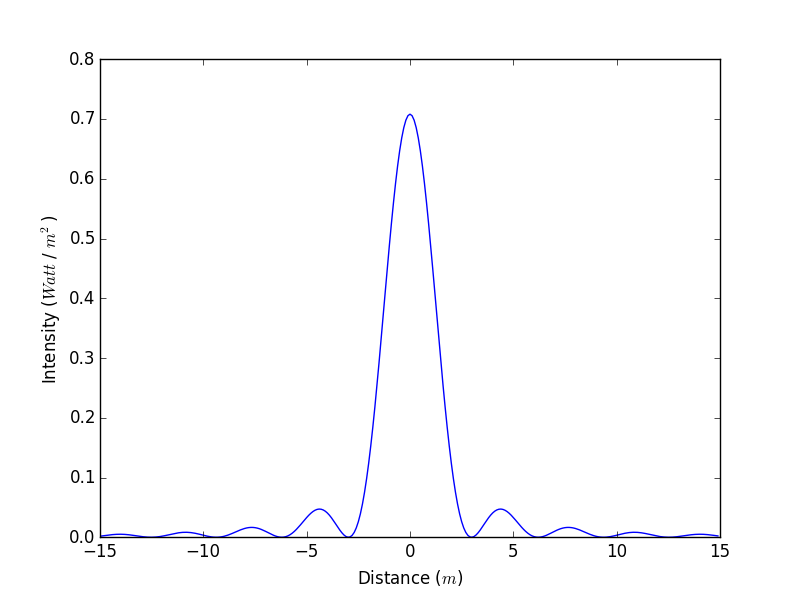
\includegraphics[scale=0.45]{figure_1.png}
\caption{Plot between distance and intensity}
\end{figure}

\begin{flushleft}
	As it should be, Intensity decreases by increasing the distance. Where at the position where source is placed we have high intensity peak.
\end{flushleft}
Next;\\
Plot between distance and intensity, for four antenna sources arrange in a linear array and by managing phase between them, we get interference pattern.
\begin{verbatim}
import numpy as np
import matplotlib.pyplot as plt
from math import sqrt, sin, pi

w=1.0
k=1.0
L=10.0 / k
P=0
# Calculate fringe spacing:
#d = 2 * 5           # Slit-spacing
#fs = 2 * pi * L / (k * d)

#print("Slit-spacing = {} produces fringe spacing = {}".format(d, fs))

ds = [-12, -4, 4, 12]
#sources=[(distance,phase)]
sources = [(-12, 0), (-4,0), (4,0), (12,0)]

def r(x,d):
return sqrt(L**2+(x-d)**2)

def Ex(x,d,p,t):
return ((x-d)/r(x,d)**2)*(sin(k*r(x,d)-w*t+p))

def Ey(x,d,p,t):
return (L/r(x,d)**2)*(sin(k*r(x,d)-w*t+p))

def I(x,sources,t):
Ox=0
Oy=0
for d, p in sources:
Ox+=Ex(x,d,p,t)
Oy+=Ey(x,d,p,t)

return Ox**2+Oy**2

def trapezoidal(f, a, b, n):
h = float(b - a) / n
s = 0.0
s += f(a)/2.0
for i in range(1, n):
s += f(a + i*h)
s += f(b)/2.0
return s * h

xs=[]
ys=[]

for x in np.linspace(-20,20,1000):
y = trapezoidal(lambda t: I(x,sources,t), -pi/w, pi/w, 100) / (2 * pi)

xs.append(x)
ys.append(y)

plt.plot(xs,ys)
plt.show()   
\end{verbatim}
\begin{figure}[ht]
	\centering	
    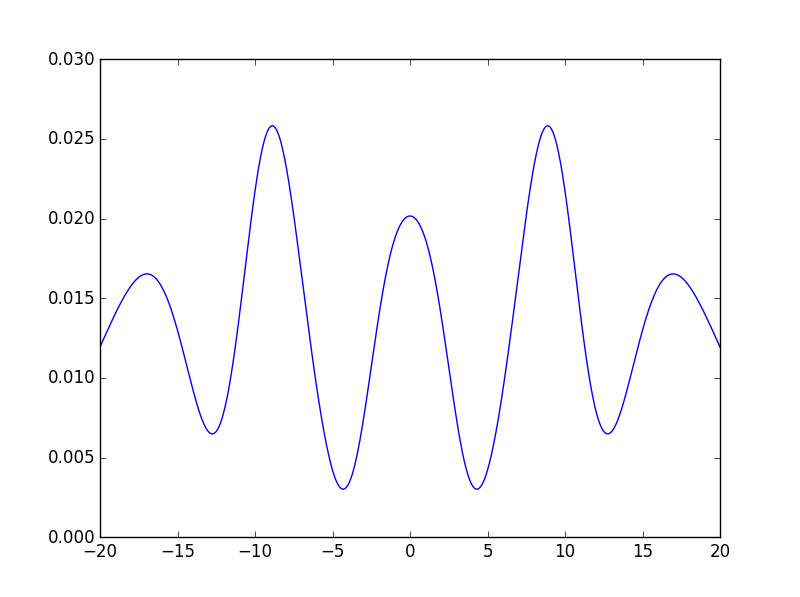
\includegraphics[scale=0.45]{figure_2.png}
	\caption{Plot between distance and intensity}
\end{figure}
